\subsection{Implementations using generic distributed frameworks}
Distributed system have already been implemented in the industry to solve the
problem of companies possessing massive amounts of data that they want to be able
to query and analyze. These frameworks largely rely on the fact that it is cheaper
to have multiple servers with relatively small storage capacity each in clusters,
than having one expensive large server.

\subsubsection{The frameworks}
The main basis of existing frameworks is based on the Google File System\cite{Grem03}. The
Google File System or GFS is the system that is used within Google to handle all
the Big data needs in the company. The architecture behind it is that all data that
is uploaded to the cluster is split up into chunks, which are then split over the
'chunk servers' in the node, and replicated a set number of times (usually 3) in
order to guarantee that data is not lost when a server/storage device breaks. The
data on the chunk servers can then be accessed by a user who contacts the master,
which knows exactly where each chunk is saved.\cite{Grem03} The Data and workflow is described
in figure \ref{GFS_Architecture} below.

\begin{figure}
  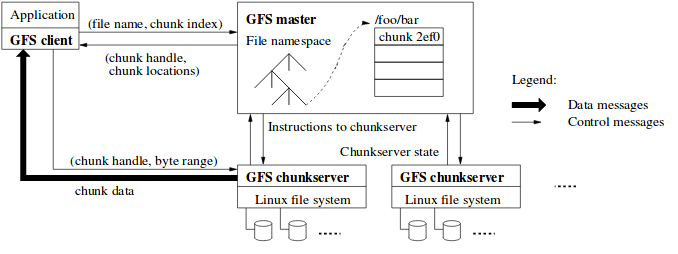
\includegraphics[scale=0.5]{GFS_Architecture.png}
  \caption{Google File System architecture\cite{Grem03}}
  \label{GFS_Architecture}
\end{figure}

The GFS architecture that was desribed in their paper by google, was adapeted into
an opensource sollution called Hadoop [2] which was worked on mainly by Yahoo! and
ditributed as an Apache project, which functions essentially the same as the GFS,
with only minor differences such as naming and chunk size. A typical use case of
adding a file to the Hadoop File System (HDFS) is show in figure \ref{Hadoop_usecase}
below.

\begin{figure}
  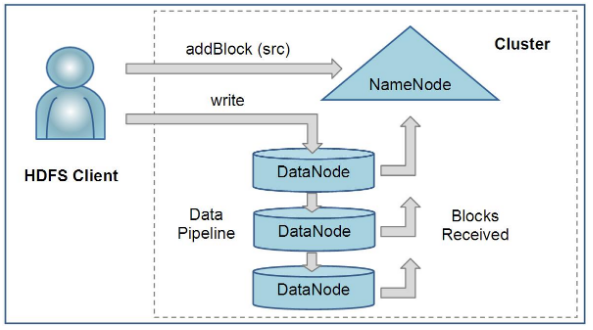
\includegraphics[scale = 0.5]{Hadoop_use_case.png}
  \caption{The data flow when adding a file to the HDFS[2]}
  \label{Hadoop_usecase}
\end{figure}

\subsubsection{Uses of the frameworks}
The storage framework highlighted above, is one of the most important basis of common implementations used today,
these implementations are the are frameworks such as Mapreduce and the Apache Spark engine.

\subsubsection{Map-reduce}
Map reduce is a new framework for processing data developed by Google[3] in order
to process data in a distributed setting, the basis behind this is that first all
data is split into tuples (called key value pairs) in the map phase, which are then passed to the reduce
phase in which a calculation is done on them to generate the desired result. The
benefit of this framework is that data can be distributed on for example a GFS or HDFS
and instead of having to pass the data to the program, each node is given the program
which is magnitudes smaller and easier to pass around. The general overview of
the execution of a map-reduce problem is given in figure \ref{mapreduce_execution}

\begin{figure}
  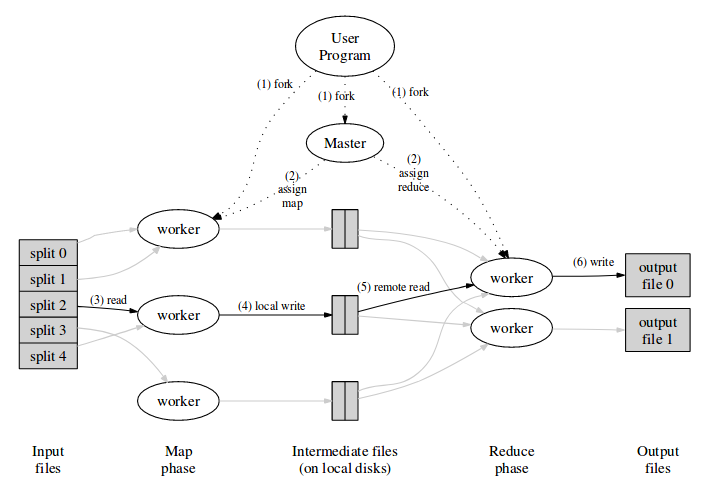
\includegraphics[scale=0.5]{mapreduce_execution.png}
  \caption{Overview of the execution of a mapreduce problem[3]}
  \label{mapreduce_execution}
\end{figure}

Furthermore the Map-reduce framework is similar to the Bulk-Synchronous processing (BSP)
style which is a little older, however, there are some difference as the Map-reduce
framework doesn't allow communication between nodes in the map phase, it does allow
communication in the reduce phase when all key value pairs are passed between workers[5].
Also, as BSP and Map-reduce are so similar work has gone into transforming BSP tasks into
map-reduce tasks and as has been shown by Goodrich et al.[4] all BSP programs can be
converted into Map-reduce programs. Other researchers have gone as far as to say
that all map-reduce task are so similar to BSP tasks that, becuase BSP has a more theoretical
basis, all tasks should be modelled as BSP tasks but implemented using the Map-reduce framework
in order to gain the speed of Map-reduce but the correctness of BSP[5].

\subsubsection{Apache Spark}
Like Map-reduce Apache Spark is another built upon the ability to run programs
on a distributed dataset. Spark is a machine learning engine that is capable of
running fully in memory[7], this has the advantage that it is a lot faster than
more traditional implementations of Hadoop program such as Map-reduce as they need
to write to disk after every step. This however does add the danger of loosing processed data
 if the power goes out in the worker node.

The way in which Spark solves the data loss problem, is to use RDDs, which are
Resilient Distributed Datasets. These datasets are read only and new ones can
only be created from storage, or merging existing RDDs[8]. The Resillient part comes
into play when the data is lost, each RDD has a lineage graph, which shows what
transformations have been executed on it. This means that once some data is lost
Spark can easily look back over the lineage graph and recalculate any lost data.
A further note must be made on the lineage graph, as they may not contain a cycle
and so be a Directed Acyclic Graph (DAG) or else data cannot be recovered.

\begin{figure}
  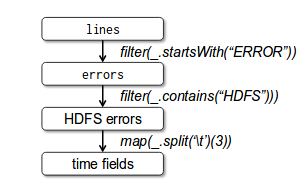
\includegraphics[scale = 0.5]{Lineage_graph.png}
  \caption{Example of the lineage graph of an RDD[8]}
  \label{lineagegraph}
\end{figure}








[2]http://storageconference.us/2010/Papers/MSST/Shvachko.pdf %HDFS paper
[3]https://static.googleusercontent.com/media/research.google.com/en//archive/mapreduce-osdi04.pdf %mapreduce paper
[4]https://arxiv.org/pdf/1101.1902v1.pdf %all bsp can be run as a map reduce problem
[5]https://arxiv.org/pdf/1203.2081.pdf %bsp vs map reduce
[6]http://www.jmlr.org/papers/volume17/15-237/15-237.pdf %MLlib and spark
[7] https://spark.apache.org/ %spark website
[8] https://www.usenix.org/system/files/conference/nsdi12/nsdi12-final138.pdf %RDD paper
